
\newpage

%=====================================================[SECTION: TWO DIMENSIONAL]
\subsection{TWO-DIMENSIONAL SYSTEMS}

In this section, the non-linear forecasting technique is expanded to series in two dimensions: space ($x$) and time ($y$). In order to rebuild the state space, lagged values in both space, $\tau_c$, and time, $\tau_r$, are used \cite{original_rubin} \cite{rubin_lagged_vals}, where again lags are found using the first minimum in the average mutual information. The technique of constructing an embedding vector is illustrated in Figure \ref{2d_method}. The top half of the image (training) is used to reconstruct the state space and forecasts are made for the bottom half of the image (testing).  In this case forecasts are made along the time axis. The forecasts are compared to the actual evolution of the system and the deterministic metric is calculated as before.

\begin{figure}[htbp]  %FIGURE
   \centering
   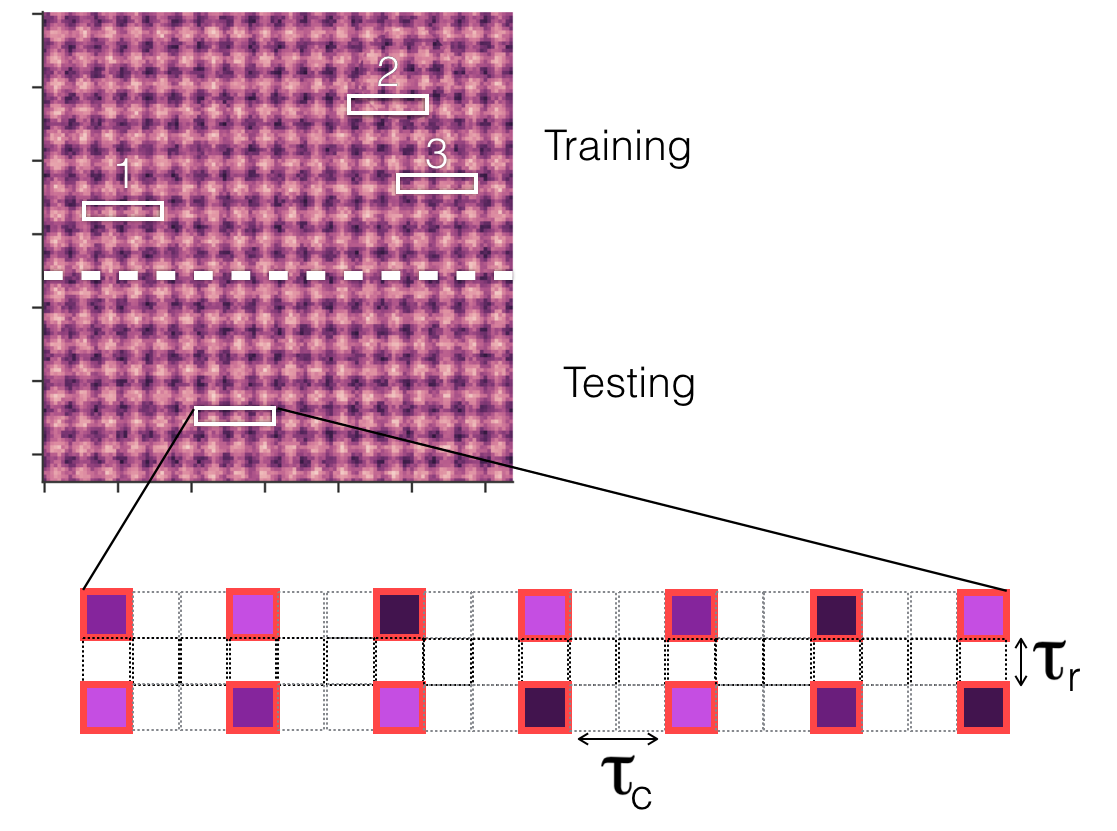
\includegraphics[width=4 in]{2d/2d_method.png} 
   \caption{Two-dimensional embedding technique. $\tau_c$ is the lag value of the columns. $\tau_r$ is lag value of the rows. The image shows an example of a fourteen-dimensional embedding. The three nearest neighbors in the training set are shown.}
   \label{2d_method}
\end{figure}

To test the technique, two-dimensional analogs of the one-dimensional series are created and analyzed. The first image (Figure \ref{spatial_logistic}) is a spatio-temporal logistic map with uncorrelated noise and is defined as:

$$x_{t+1} = Ax_t(1-x_t)\equiv f(x_t)$$

$$x_{t+1,s} = \frac{1}{1+4\epsilon}[f(x_{t,s})+\epsilon f(x_{t,s\pm1}) + \epsilon f(x_{t,s\pm2})] +\alpha\eta.$$

Where $x$ is the series being generated, $A$ is a constant, $f$ is the logistic function, $\epsilon$ parameterizes the spatial coupling, $\alpha$ is the amplitude of the noise, and $\eta$ is uncorrelated noise between zero and one. The second image is a periodic function in space added to a periodic function in time with uncorrelated noise added(Figure \ref{spatial_periodic}). The noise amplitude, $alpha$, is increased incrementally for both images and the trends of the $R^2$ values are analyzed over a range of near neighbors and forecast distances.

\begin{figure}[htbp]  %FIGURE
   \centering
   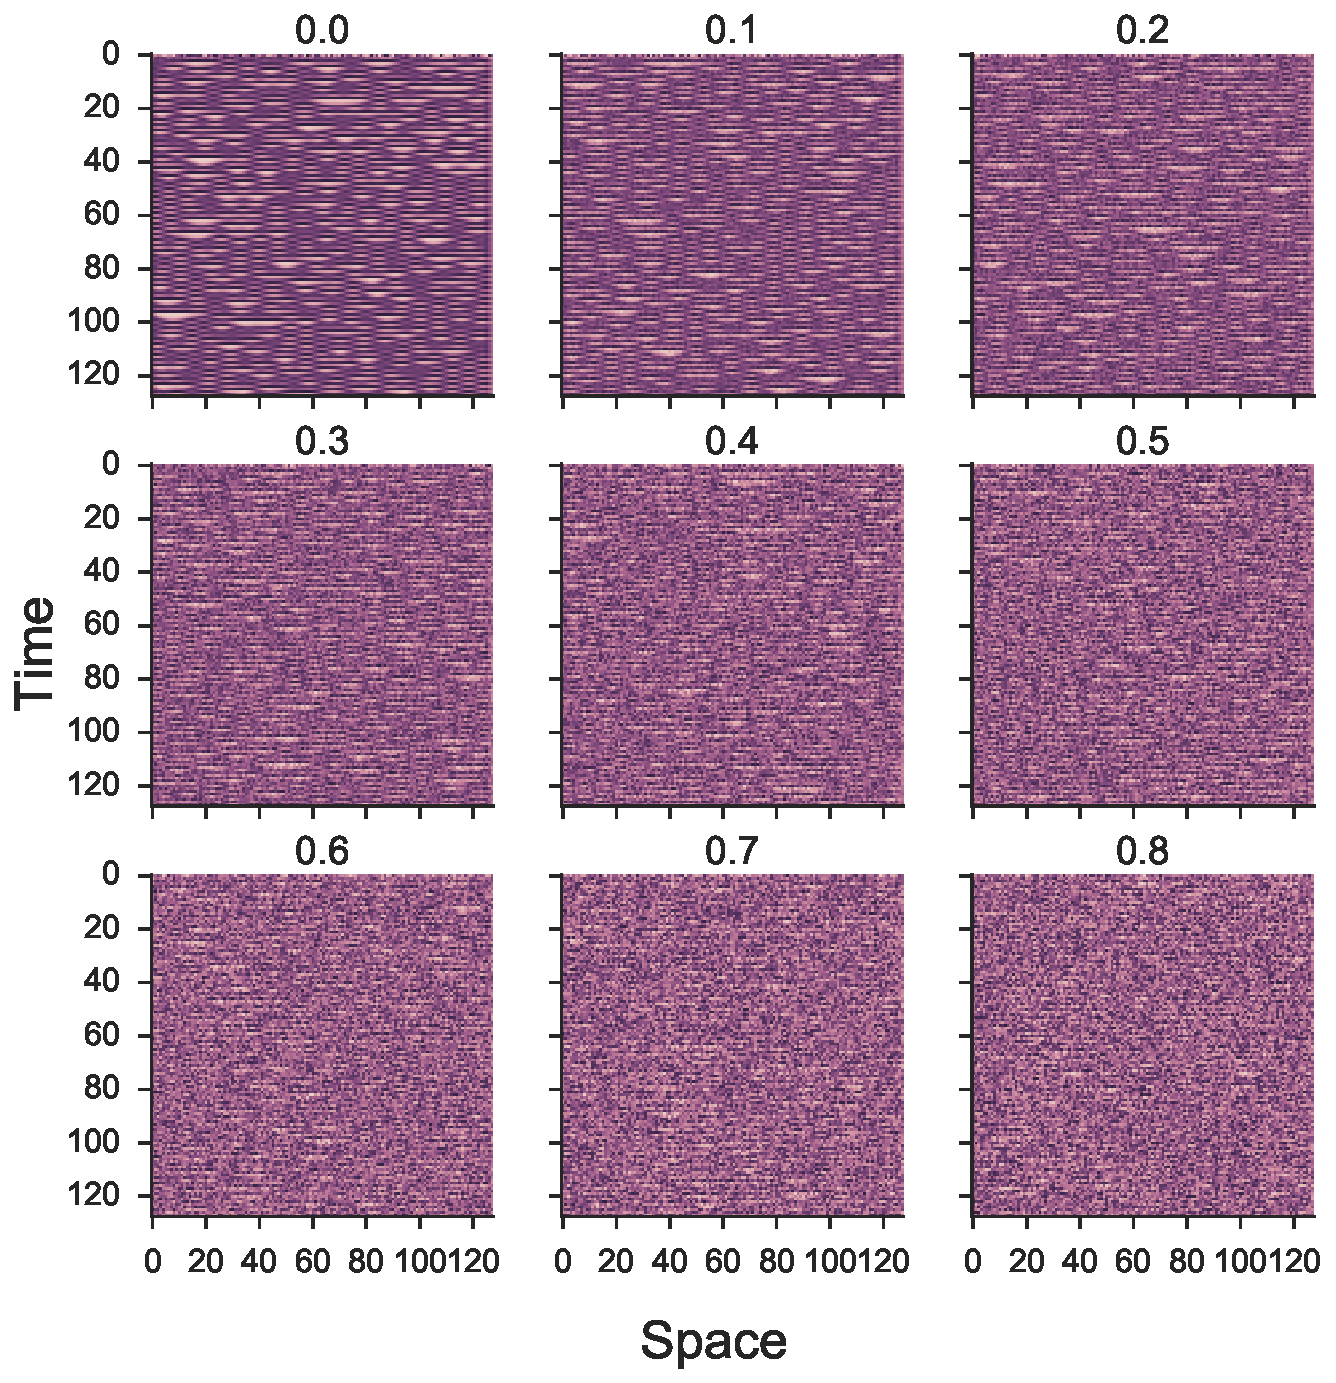
\includegraphics[width=4 in]{2d/chaosNoiseLevels.pdf} 
   \caption{Two-dimensional logistic map. The number on the plot indicates the amplitude of the added noise, $\alpha$. }
   \label{spatial_logistic}
\end{figure}

\begin{figure}[htbp]  %FIGURE
   \centering
   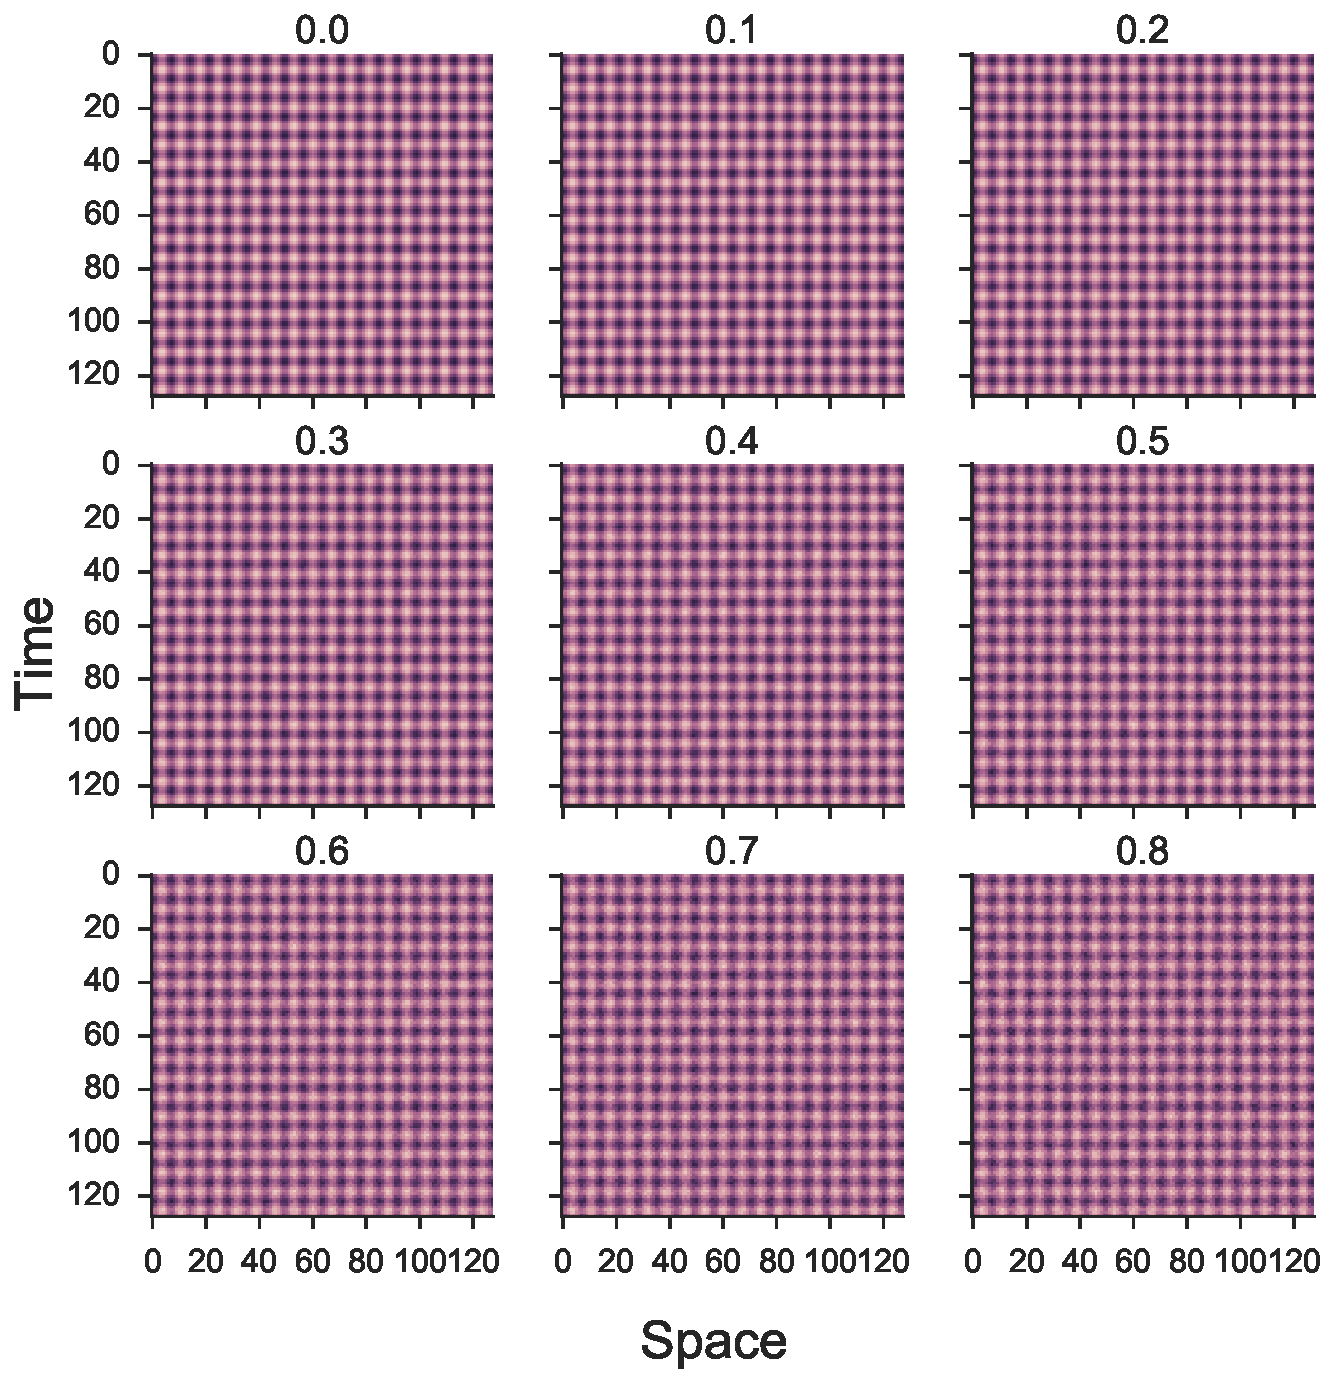
\includegraphics[width=4 in]{2d/periodic_noise.pdf} 
   \caption{Two-dimensional periodic image. The number on the plot indicates the amplitude of the added noise, $\alpha$.}
   \label{spatial_periodic}
\end{figure}


The spatio-temporal non-linear forecasting technique is applied to each of the generated images. The results for the spatio-temporal chaotic image and spatio-temporal periodic image are shown in Figure \ref{spatial_logistic_contour} and Figure \ref{spatial_periodic_contour} respectively.


\begin{figure}[htbp]  %FIGURE
   \centering
   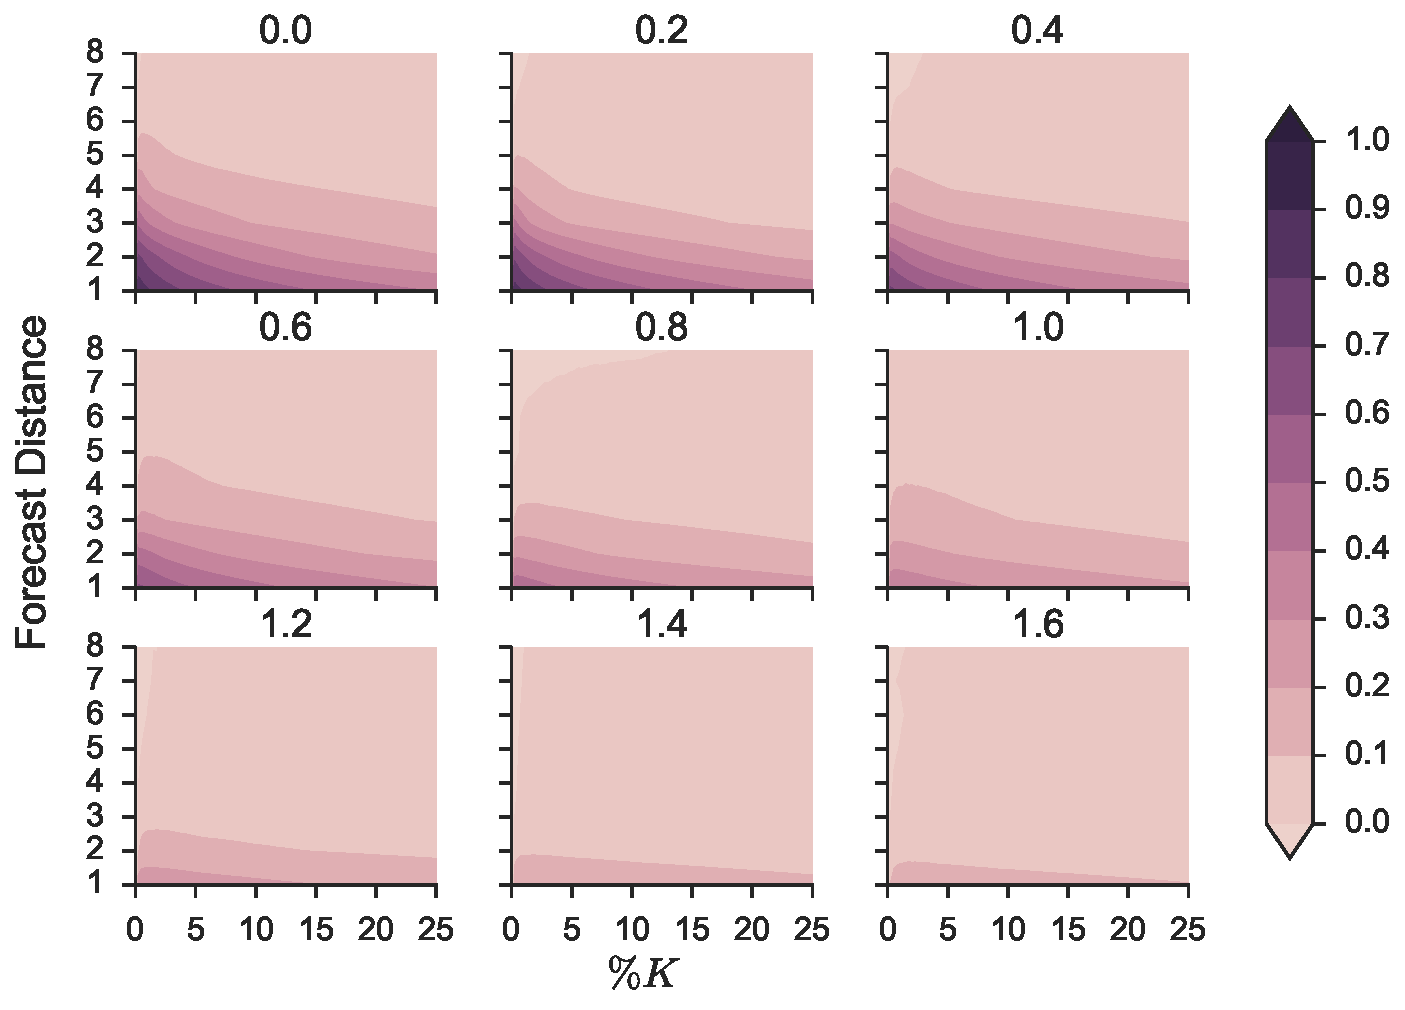
\includegraphics[width=4 in]{2d/chaos_noise_contours.pdf} 
   \caption{Non-linear forecasting results for the spatio-temporal logistic map with different amplitudes of noise. The coefficient of determination, $R^2$, is plotted against near neighbors ($K$) and forecast distance. The number on the plot indicates the amplitude of the noise, $\alpha$.}
   \label{spatial_logistic_contour}
\end{figure}

\begin{figure}[htbp]  %FIGURE
   \centering
   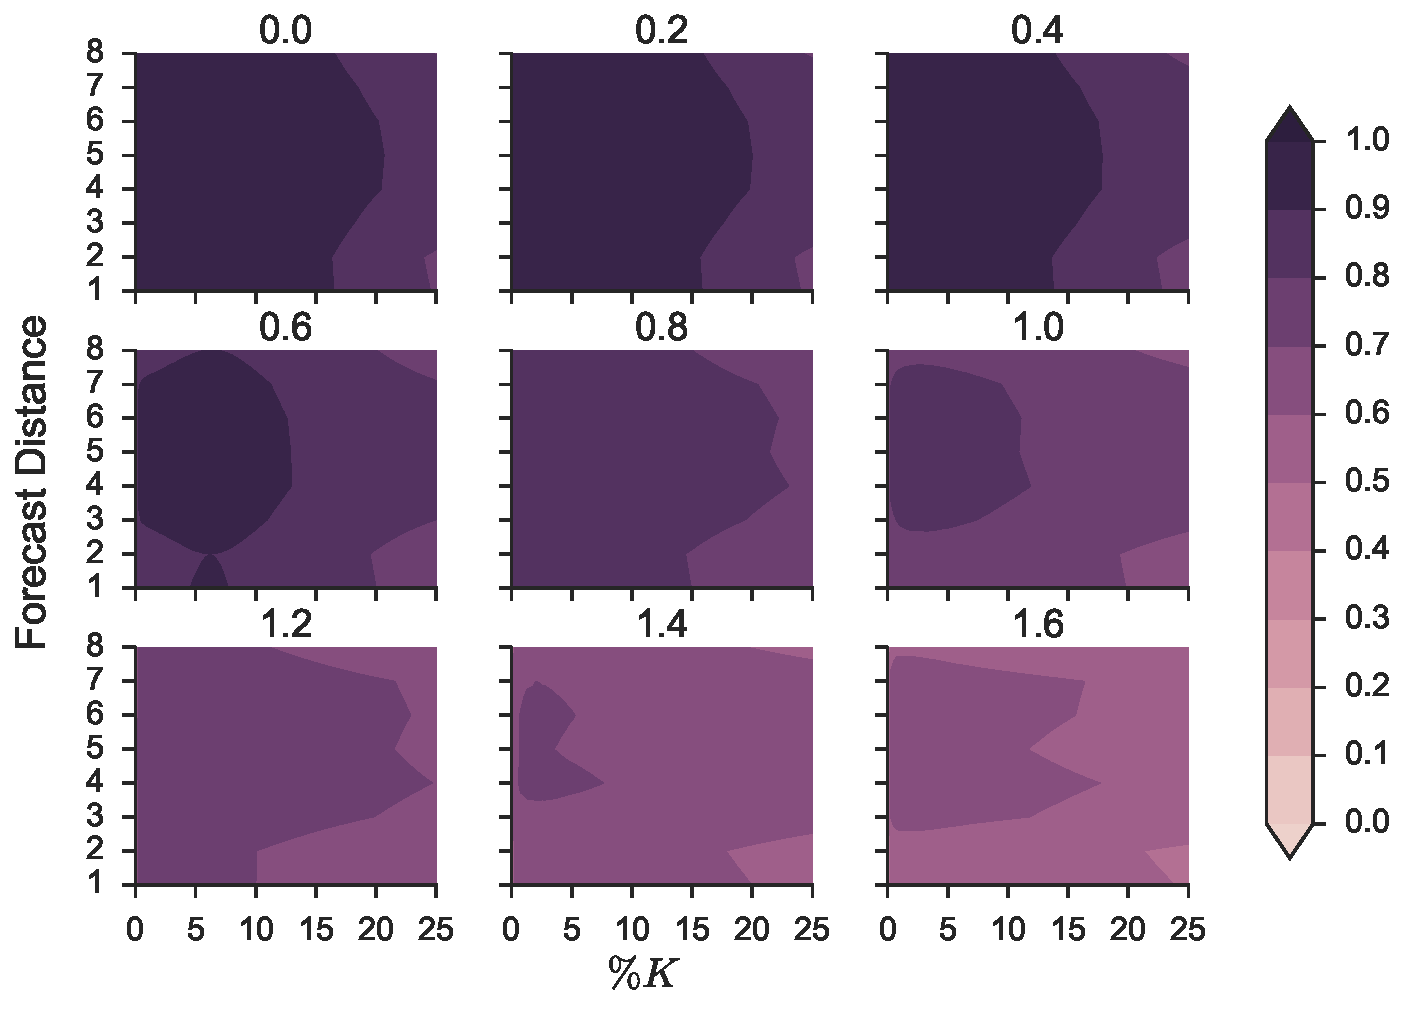
\includegraphics[width=4 in]{2d/periodic_noise_contours.pdf} 
   \caption{Non-linear forecasting results for the spatio-temporal periodic image with different amplitudes of noise. The coefficient of determination, $R^2$, is plotted against near neighbors ($K$) and forecast distance. The number on the plot indicates the amplitude of the noise, $\alpha$.}
   \label{spatial_periodic_contour}
\end{figure}

For both systems, the results of using the non-linear forecasting analysis are similar to the one-dimensional systems. For the spatio-temporal chaotic map, high $R^2$ values are obtained at low $K$ values and low forecast distances. This trend is present across all levels of noise and illuminates the nonlinear deterministic dynamics in the system and the sensitivity to initial conditions. Additionally, the two-dimensional periodic image preserves the trends of the one-dimensional periodic equation. Forecast skill does not noticeably decrease with increasing forecast distance and decreases slowly with number of neighbors used to forecast.

The deterministic metric is calculated for each of the contours and the results are shown for the chaotic image and the periodic image in Figures \ref{spatial_logistic_metric} and \ref{spatial_periodic_metric}.

\begin{figure}[htbp]  %FIGURE
   \centering
   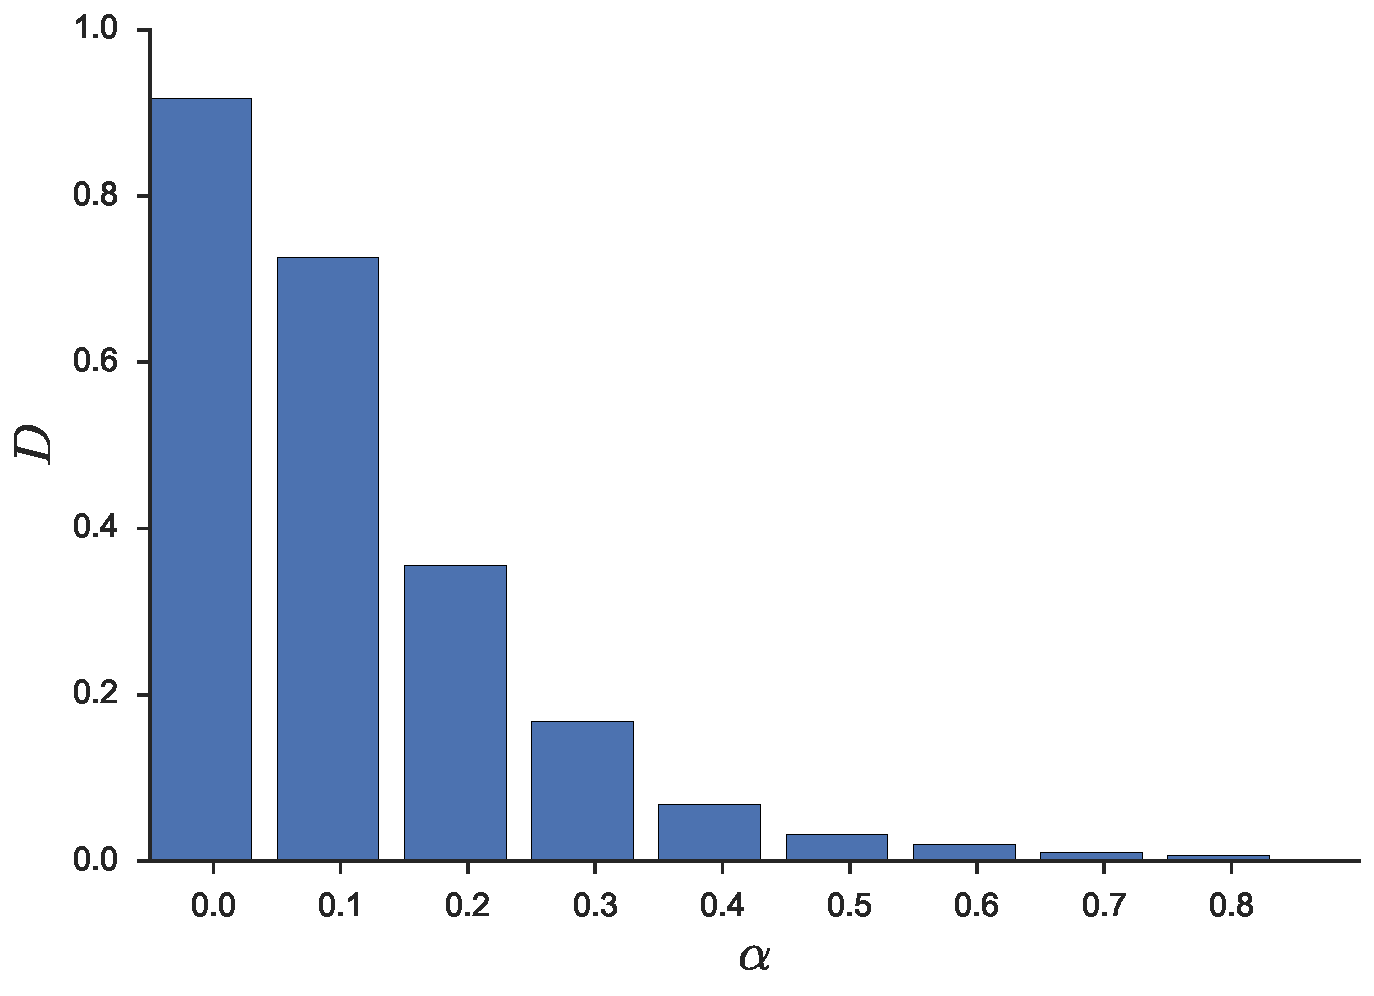
\includegraphics[width=4 in]{2d/chaotic_bar_plot.pdf} 
   \caption{Deterministic metric for the spatio-temporal logistic map. The $x$-axis indicates the amplitude of the noise, $\alpha$.}
   \label{spatial_logistic_metric}
\end{figure}

\begin{figure}[htbp]  %FIGURE
   \centering
   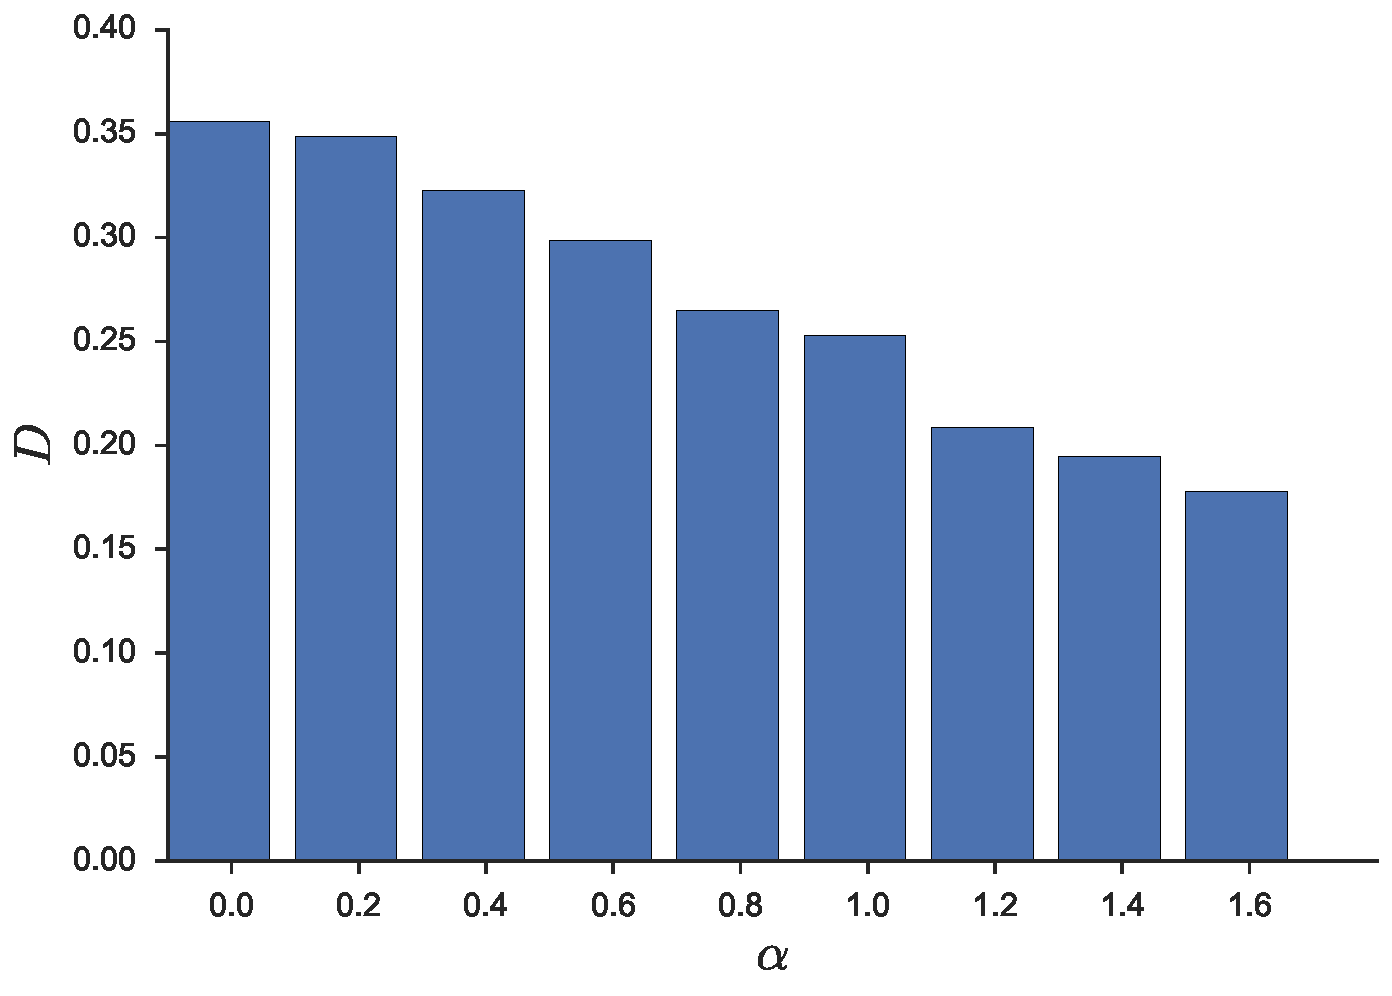
\includegraphics[width=4 in]{2d/periodic_bar_plot.pdf} 
   \caption{Deterministic metric for the two-dimensional periodic image. The $x$-axis indicates the amplitude of the noise, $\alpha$.}
   \label{spatial_periodic_metric}
\end{figure}





The trends in $D$ as noise is added to the system illustrate the effectiveness of the metric in spatio-temporal images. Systems that are more deterministic (less noise) have higher $D$ values and systems that are more stochastic (more noise) have lower $D$ values. Again, it is important to note that the metric is not able to cross over systems with different system dynamics. Comparing $D$ values for a system with periodic dynamics to a system with chaotic dynamics is not useful.



% %====================================================[subsection: Discrete spaces]
\subsection{DISCRETE SPACES}

The two-dimensional technique is extended to discrete images where each pixel belongs to a class. Images of two different stochastic systems are analyzed (Figure \ref{discrete_maps}). The first image is randomly placed circles of different sizes where the majority of the space is a single class (light blue). The second image is voronoi polygons where each class is equally represented in the space and each is roughly the same size.

\begin{figure}[htbp]  %FIGURE
   \centering
   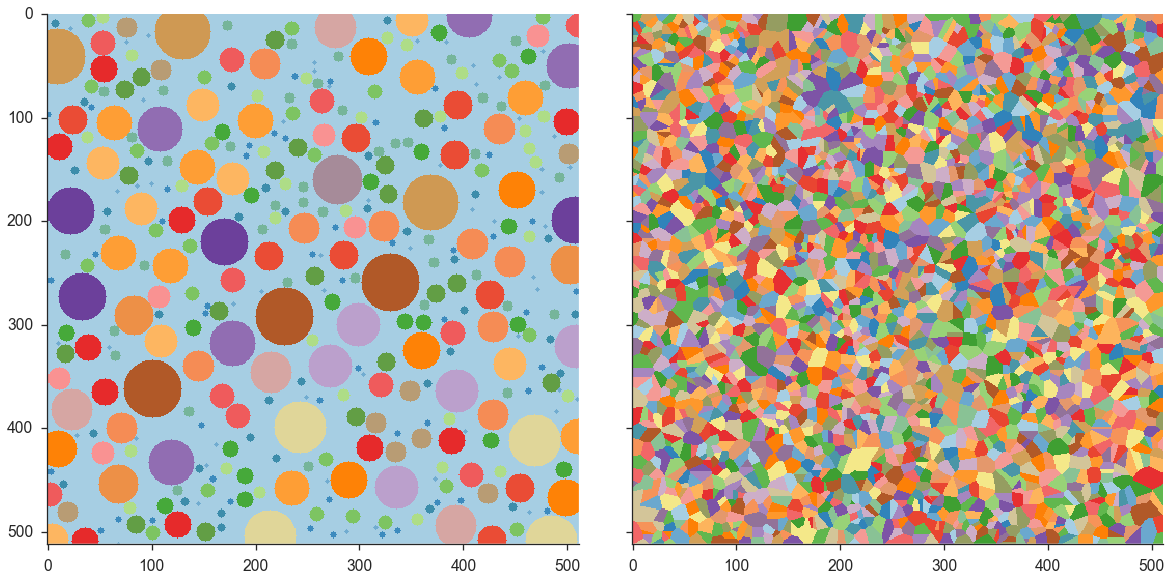
\includegraphics[width=4 in]{2d/discrete_spaces.png} 
   \caption{Left: Randomly placed circles of varying size. Right: Voronoi polygons. Color in both images corresponds to class.}
   \label{discrete_maps}
\end{figure}

In order to apply the non-linear forecasting technique, some modifications are necessary. First, rather than computing the $R^2$ value when making forecasts, the percent correctly forecast is calculated as:

$$ P_c = \frac{ N_c}{ N_t},$$

where $P_c$ is the percent correct, $N_c$ is the number correctly forecast, and $N_t$ is the total number of forecasts. Second, the hamming distance between two points in the state space is calculated instead of the euclidean distance. This is to account for classes being discrete labels and not continuous values. Figure \ref{discrete_contours} shows contours of the percent correct for each surrogate image when using the nonlinear forecasting technique adjusted for discrete data. 

\begin{figure}[htbp]  %FIGURE
   \centering
   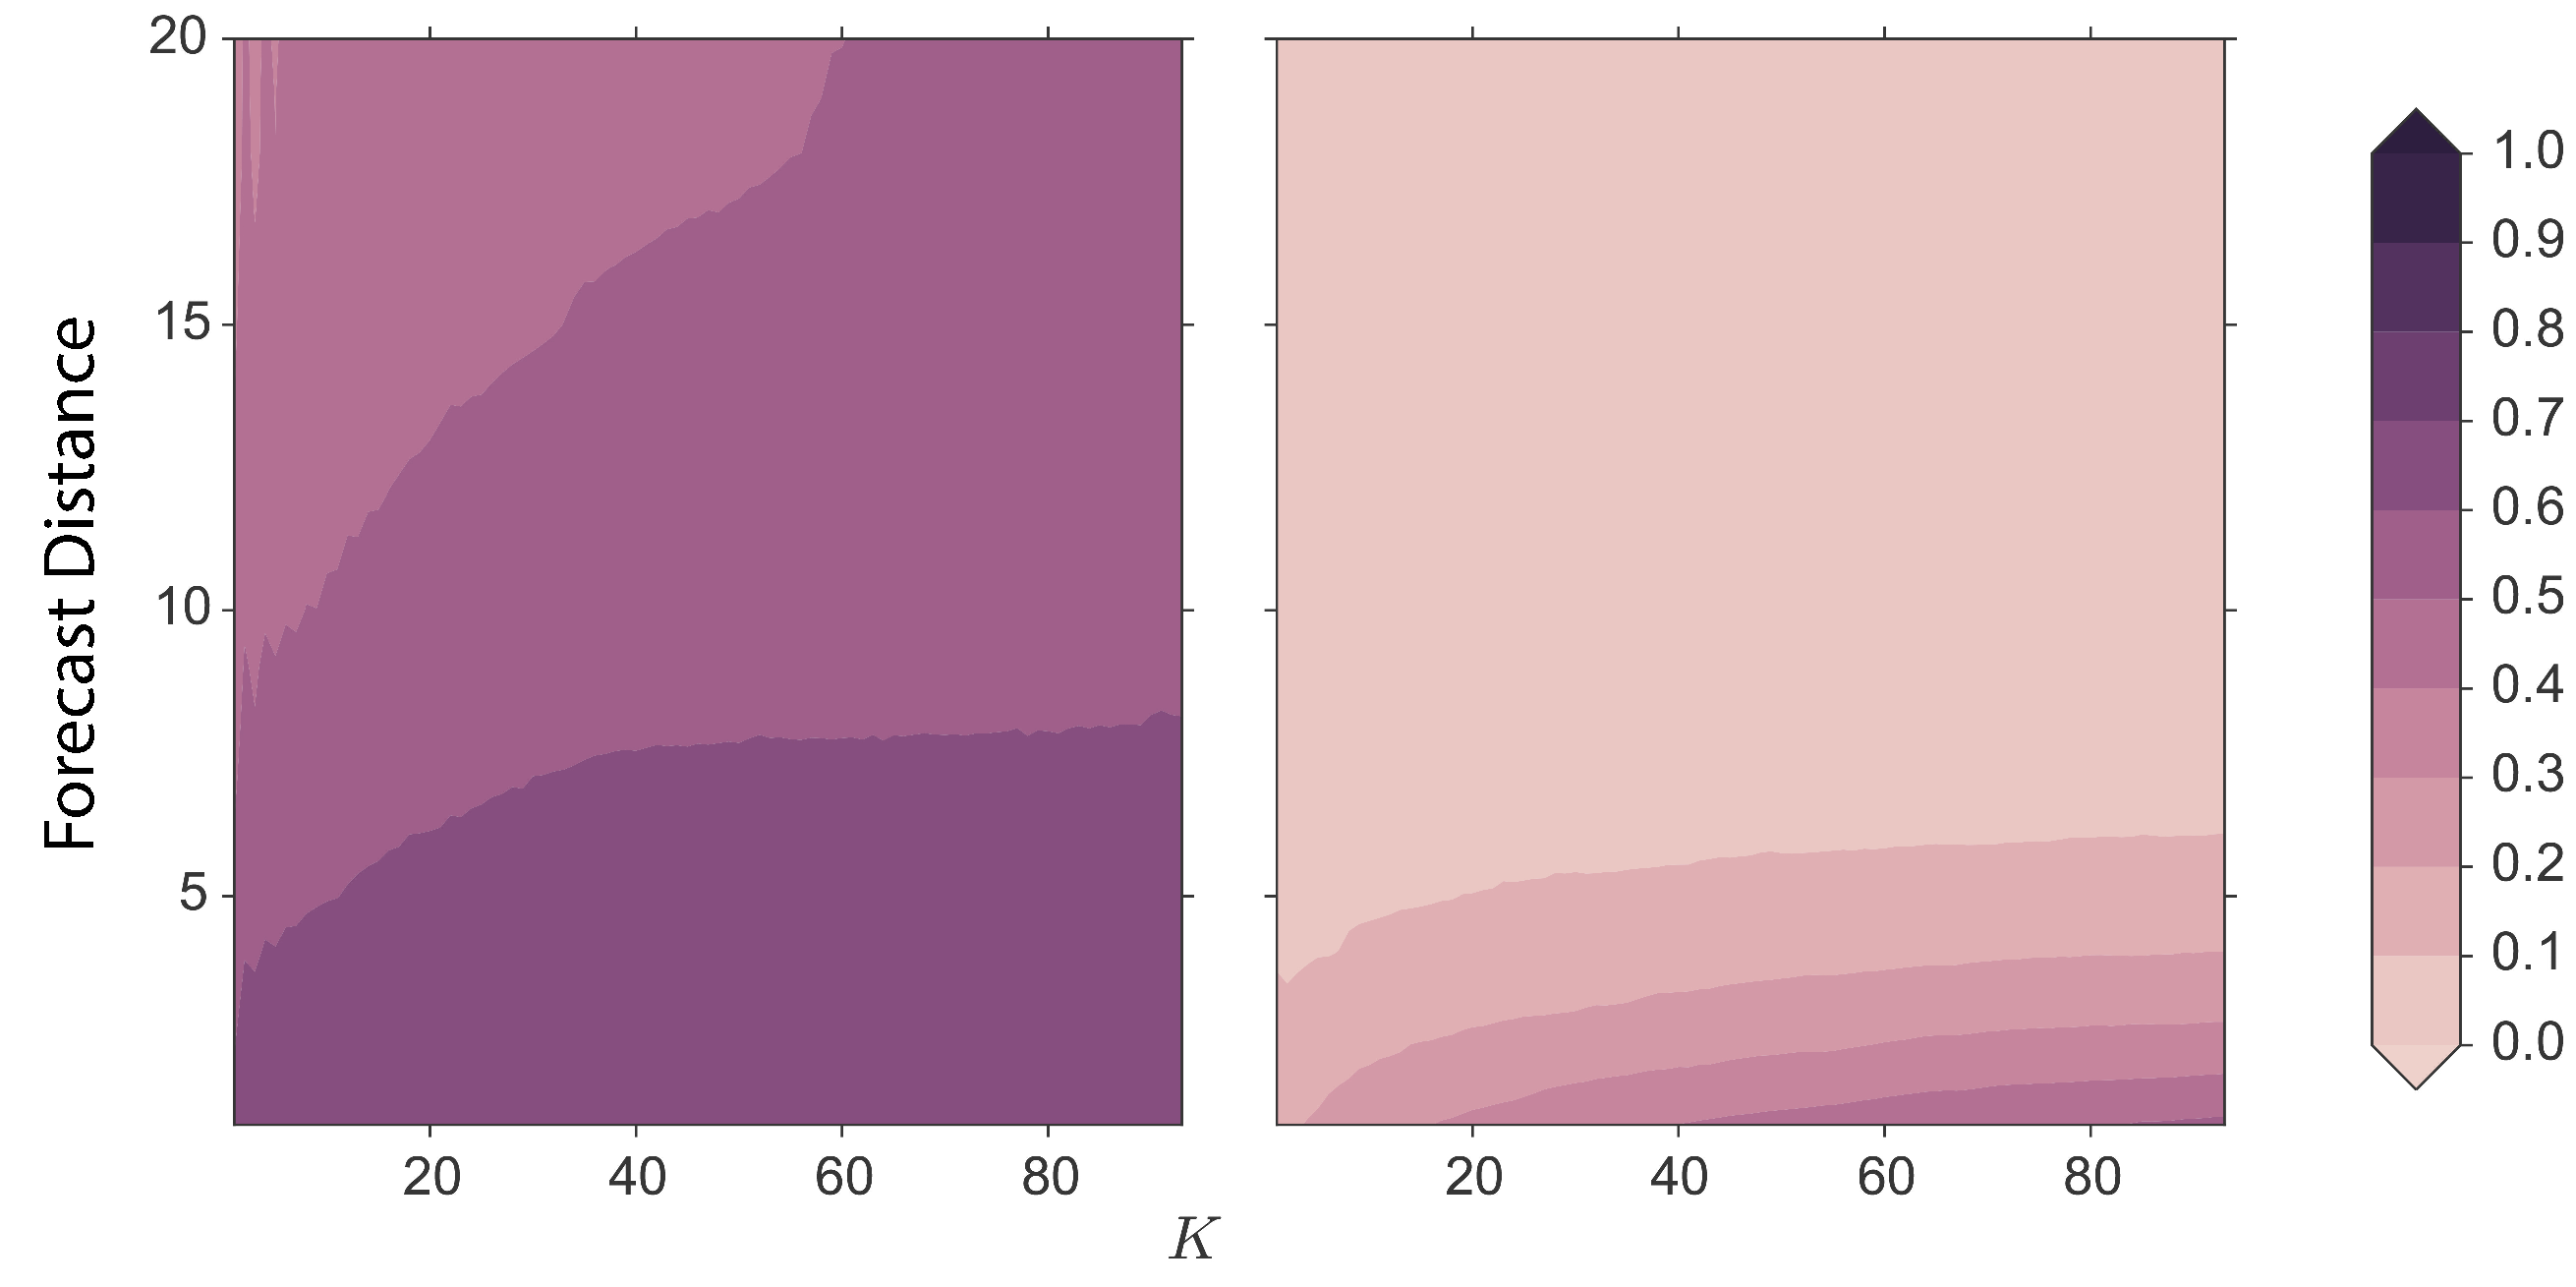
\includegraphics[width=4 in]{2d/discrete_contours.pdf} 
   \caption{Non-linear forecasting results for the random circles (left) and voronoi polygons (right). The coefficient of determination, $R^2$, is plotted against near neighbors ($K$) and forecast distance.}
   \label{discrete_contours}
\end{figure}

For both images, forecast skill increases as $K$ increases indicating that both systems are not deterministic. Averaging larger amounts of near neighbors results in better forecast skill and thus near neighbors in the reconstructed space do not evolve similarly. Additionally, forecast skill decreases as forecast distance increases. The trend, however, is not due to chaotic dynamics and is instead due to the high autocorrelation of the images coupled with its stochastic structure. Specifically, the autocorrelation causes high $P_c$ values at low forecast distances, but the stochasticity causes higher forecast distances to result in lower $P_c$ values. For the randomly dropped circles, averaging additional trajectories results in a forecast of the mode of the space (light blue). For the voronoi polygons, $P_c$ drops to zero at a forecast distance of five pixels, which is roughly the radius of the polygons.

While there is no comparison here of the deterministic metric along a gradient of noise, the patterns associated with stochastic systems are present: increasing forecast skill with increasing $K$ values. Moreover, both images produce a negative deterministic metric indicating that the system is stochastic.







